\documentclass[12pt]{article}
\usepackage[utf8x]{inputenc}
\usepackage{amsmath}
\usepackage{multicol}
\usepackage{graphicx}
\usepackage{float}
\usepackage{dsfont}
\usepackage{textcomp}
\usepackage{multirow}
\usepackage{amsfonts}
\usepackage{cleveref}
\usepackage{fancyhdr}
\setlength{\headheight}{14.5pt}
\renewcommand{\sectionmark}[1]{\markright{#1}{}}
\usepackage[T1]{fontenc}
\usepackage[colorinlistoftodos]{todonotes}
\usepackage[margin=2cm,a4paper]{geometry}
\newgeometry{left=2.0cm,right=2.0cm,top=2.5cm,bottom=2.5cm}
\usepackage{listings}
\setlength{\marginparwidth}{2cm}
\setlength{\parindent}{0pt}
\newcommand{\deriv}{\mathrm{d}}
\lstset{
    language=R,
    basicstyle=\scriptsize\ttfamily,
    commentstyle=\ttfamily\color{red},
    numbers=left,
    numberstyle=\ttfamily\color{blue}\footnotesize,
    stepnumber=1,
    numbersep=5pt,
    backgroundcolor=\color{white},
    showspaces=false,
    showstringspaces=false,
    showtabs=false,
    frame=single,
    tabsize=2,
    captionpos=b,
    breaklines=true,
    breakatwhitespace=false,
    title=\lstname,
    escapeinside={},
    keywordstyle={},
    morekeywords={}
    }
\title{}
\pagestyle{fancy}
\fancyhf{}
\rhead{\leftmark}
\lhead{Nuclear Magnetic Resonance}
\lfoot{PH617 Physics Project Laboratory}
\rfoot{Page \thepage}
\renewcommand{\headrulewidth}{1pt}
\renewcommand{\footrulewidth}{1pt}
\begin{document}
\begin{titlepage}
\newgeometry{left=1.0in,right=1.0in,top=2.0in,bottom=2.0in}
\newcommand{\HRule}{\rule{\linewidth}{0.5mm}}
\begin{centering} 
%---------------------------------------------------------------------------
%	HEADING SECTIONS
%---------------------------------------------------------------------------

\includegraphics[scale=0.7]{Images/Uni_of_Kent.png}\\[1cm]
%---------------------------------------------------------------------------
%	TITLE SECTION
%---------------------------------------------------------------------------
\HRule \\ [0.3cm]
\Huge{\bfseries{Nuclear Magnetic Resonance}} \\
\textsc{\large PH617: Physics Project Laboratory}\\ [-0.1cm]
\textsc{\large Astronomy, Space Science and Astrophysics}\\ [-0.2cm]
\HRule \\[0.5cm]
%---------------------------------------------------------------------------
%	AUTHOR SECTION
%---------------------------------------------------------------------------
\begin{minipage}{0.625\textwidth}
\begin{center} \large
{\large Date: 13th Nov 2020 - 2nd Dec 2020}\\[0.2cm]
{\large Report Author: Lukasz R Tomaszewski}\\[0.2cm]
{\large Word Count: 1994}\\
\end{center}
\end{minipage}\\[2cm]
\vfill
\end{centering} 
\end{titlepage}
%---------------------------------------------------------------------------
%	CONTENTS   
%---------------------------------------------------------------------------
\newpage
\begin{titlepage}
\begin{tableofcontents}
\end{tableofcontents}
\end{titlepage}
\newpage
%---------------------------------------------------------------------------
%	ABSTRACT
%---------------------------------------------------------------------------
\section{Abstract}
\label{Abstract Section}

Nuclear Magnetic Resonance (NMR) is used to observe nuclei in a materials structure, this experiment explore NMR and calculates the line-width of glycerine at 4.422 kHz and shows the use of NMR in chemistry and biology by pre-setting the nuclei that requires detecting. The g-factor is determined as $-5.37$ from experimental data but failed to compare to a literature value of $-5.05x10^{-3}$. Though analysis shows that apparatus restrictions prevented more detailed results and in depth analysis.

%---------------------------------------------------------------------------
%	INTRODUCTION
%---------------------------------------------------------------------------
\section{Introduction}
\label{Introduction Section}

Since its discovery in 1945 by Felix Bloch and Edward Purcell, Nuclear Magnetic Resonance (NMR) has been used to probe and observe the structure of materials by measuring nuclei. It's used in all areas of science: Physics, Chemistry and Biology, in Physics and Chemistry its used to measure how the nuclei reacts to an external magnetic field by observing the interactions of atomic nuclear spins. In Biology it's referred to as magnetic resonance imaging (MRI) where utilising strong magnetic fields to highlight human anatomy without penetrating tissue. Within this experiment different materials will be placed inside a magnetic field to where a Nuclear Magnetic Resonance (NMR) signal will be detected, where the the Full Width Half Maximum (FWHM) will be calculated and compared to the $T_2$ relaxation of Glycerine. To which will lead on to determine the g factor to both Glycerine and PTFE, then ultimately show how Nuclear Magnetic Resonance (NMR) is used in all areas of science and discuss its benefits. \\ 

The aims are to create an experiment and observe this and to; \cite{Exp.A-2020}

\begin{itemize}
    \item Nuclear Magnetic Resonance on protons and fluorine in a liquid and solid samples.
    \item Determination of the line width of the $'^$H resonance.
    \item Determination of the g-factor for the protons and fluorine.
\end{itemize}

%---------------------------------------------------------------------------
%	METHODOLOGY
%---------------------------------------------------------------------------
\section{Methodology}
\label{Methodology Section}

%---------------------------------------------------------------------------
\subsection{Experimental Setup}
\label{Experimental Setup Subsection}

%---------------------------------------------------------------------------
\subsubsection{Physical NMR Spectroscopy}
\label{Physical NMR Spectroscopy SubsubSection}

By setting up the equipment using the apparatus list shown in \cite{Exp.A-2020}, the PicoScope software is used to shown the waveform on the Nuclear Magnetic Resonance (NMR) on a computer. Different materials are placed approximately 15mm into the centre of the magnetic field so that the nuclei will be affected by the surround magnetic field equally thus allowing a stable measurement of the Nuclear Magnetic Resonance (NMR) signal to be detected. The materials are Glycerine, Water, Polystrene and Polytetrafluorethylene (PTFE), a Nuclear Magnetic Resonance (NMR) signal will be detected for each material to analysis the behaviour of the magnetic field on the materials nuclei and how the change in amplitude and frequency alters the NMR waveform. The Full Width Half Maximum of Glycerine will be calculated and compared to the $T_2$ relaxation using \cref{Log Tramsittance}.

\begin{equation}
\Delta v= \dfrac{1}{T_2}
\label{Log Tramsittance}
\end{equation}

%---------------------------------------------------------------------------
\subsubsection{Chemical NMR Spectroscopy}
\label{Chemical NMR Spectroscopy SubsubSection}

Much like in \cref{Physical NMR Spectroscopy SubsubSection}, the observation of the Nuclear Magnetic Resonance (NMR) signal of hand cream will be detected, utilising the Glycerine material. The PicoScope will be be calibrated to observe a Glycerine NMR signal as the hand cream contains glycerine, the NMR signal will only pick up on the glycerine signal in the hand cream with only minor or no alteration to the amplitude or frequency. This part of the experiemnt will prove the Nuclear Magnetic Resonance (NMR) use in Chemistry to pick up certain chemical elements inside materials.

%---------------------------------------------------------------------------
\subsubsection{Biological NMR Spectroscopy}
\label{Biological NMR Spectroscopy SubsubSection}

Again much like in \cref{Chemical NMR Spectroscopy SubsubSection}, the Nuclear Magnetic Resonance (NMR) signal of water will be observed first and then a fresh piece of cut grass shall be place into the magnetic field in which the PicoScope shall only detect the water molecules inside the fresh cut grass. This experiment will show how Nuclear Magnetic Resonance (NMR) signals are used to observe specific molecules inside materials. Ultimately will also prove some understanding on how Magnetic Resonance Imaging (MRI) works and the advancements in medical science Nuclear Magnetic Resonance (NMR) has done. 

%---------------------------------------------------------------------------
\subsubsection{Determination of the g-factor}
\label{Determination of the g-factor SubsubSection}

For the final segment of this experiment, the glycerine and Polytetrafluorethylene (PTFE) samples will be placed into the magnetic field again and their Nuclear Magnetic Resonance (NMR) signal be observed, this time changing not only the amplitude and frequency but the current of the magnetic field as well. The change in current should show a correlation with frequency and ultimately a relationship between frequency and the magnetic field strength, once the Nuclear Magnetic Resonance (NMR) signal is found by re calibrating the amplitude and frequency the sample is taken out and replaced with a Combi B-sensor S \cite{Exp.A-2020} which will measure the strength of the magnetic field. Multiple measurements will be taken and plotted to which the gradient of the linear line of fit with give the value for both samples g-factors.

%---------------------------------------------------------------------------
%	REPORT & FINDINGS
%---------------------------------------------------------------------------
\section{Results \& Findings}
\label{Results & Findings Section}

%---------------------------------------------------------------------------
\subsection{Physical NMR Spectroscopy}
\label{Physical NMR Spectroscopy SubSection}

By collecting the frequency, current and voltage of each of the four samples (glycerine, water, polystyrene and PTFE) shown in \cref{Phy NMR Spec} utilising the experiment set up in \cref{Physical NMR Spectroscopy SubsubSection} shows a strong relationship between the samples, by varying the frequency gives the Nuclear Magnetic Resonance (NMR) signal and adjusting the RF amplitude gives the best signal/ noise ratio, this is shown in \cref{Part 1 1A}. By then plotting the voltage against the magnetic field strength for each material in \cref{Part 1 1B} for the glycerine sample, \cref{Part 1 2B} for the water sample, \cref{Part 1 3B} for the polystyrene sample and \cref{Part 1 4B} for the PTFE sample. This improved graph shows how the Nuclear Magnetic Resonance (NMR) signal is affected for each sample at different strength of the magnetic field.

\begin{table}[H]
\begin{center}
 \footnotesize
 \begin{tabular}{|c||c||c||c||c|}
 \hline
 \multicolumn{5}{|c|}{Nuclear Magnetic Resonance (NMR) of protons in liquid and solid samples} \\
 \hline
 Material & Frequency (MHz)  & Current (Amps)  & Voltage (V) & Standard Deviation \\
 \hline \hline
 Glycerine & 17.6460 $\pm$0.0001  & 3.15 $\pm$0.01  & 7.5 $\pm$0.1 & 7.439\\
 \hline
 Water & 17.7579 $\pm$0.0001  & 3.17 $\pm$0.01  & 7.6 $\pm$0.1 & 7.479\\
 \hline
 Polystyrene & 17.8296 $\pm$0.0001 & 3.16  $\pm$0.01  & 7.9 $\pm$0.1 & 7.486\\
 \hline
 PTFE & 17.6947 $\pm$0.0001  & 3.17 $\pm$0.01  & 7.8  $\pm$0.1 & 6.874\\
 \hline
 \end{tabular} \\ 
 \caption{List of variable data collected from different liquid and solid samples when using NMR to detect protons.}
 \label{Phy NMR Spec}
\end{center}
\end{table}

Determining the line-width of the glycerine Nuclear Magnetic Resonance (NMR) signal, will utilise the PicoScope software, as in \cite{Exp.A-Lab_book} two values were selected in the wave in \cref{Linewidth} and the difference in voltage as well, which were put into \cref{FWHM 1} and resulted in \cref{FWHM 2}. Within this calculation the values change from volts to Hertz, or voltage to frequency for better clarity of the Full Width Half Maximum and will allow comparison for the line width calculation of the $T_2$ relaxation of glycerine of 18ms, the new $\Delta v$ is calculated using \cref{Log Tramsittance} and results in \cref{T2}. Full calculations found in \cite{Exp.A-Lab_book}\\

\begin{equation}
\Delta f = q * \Delta v
\label{FWHM 1}
\end{equation}

\begin{equation}
\Delta f = 23787.5 Hz/v * 0.001859v = 4.422 kHz
\label{FWHM 2}
\end{equation}

\begin{equation}
\Delta f = 3428.83 Hz/v * 0.001859v = 637.42 Hz
\label{T2}
\end{equation}

The line width of \cref{FWHM 2} compared to \cref{T2} is significantly larger, mostly due to the fact that the experimental setup used to record the data show in \cref{Part 1 1A} as the many protons occupying the many nuclei fall under the scope of one fairly small magnetic field whereas in a more sophisticated experimental environment would allow for the one stronger magnetic field to be used and the detection of the individual protons for the many nuclei in the Nuclear Magnetic Resonance (NMR) signal. \\

\begin{figure}[H]
\centering
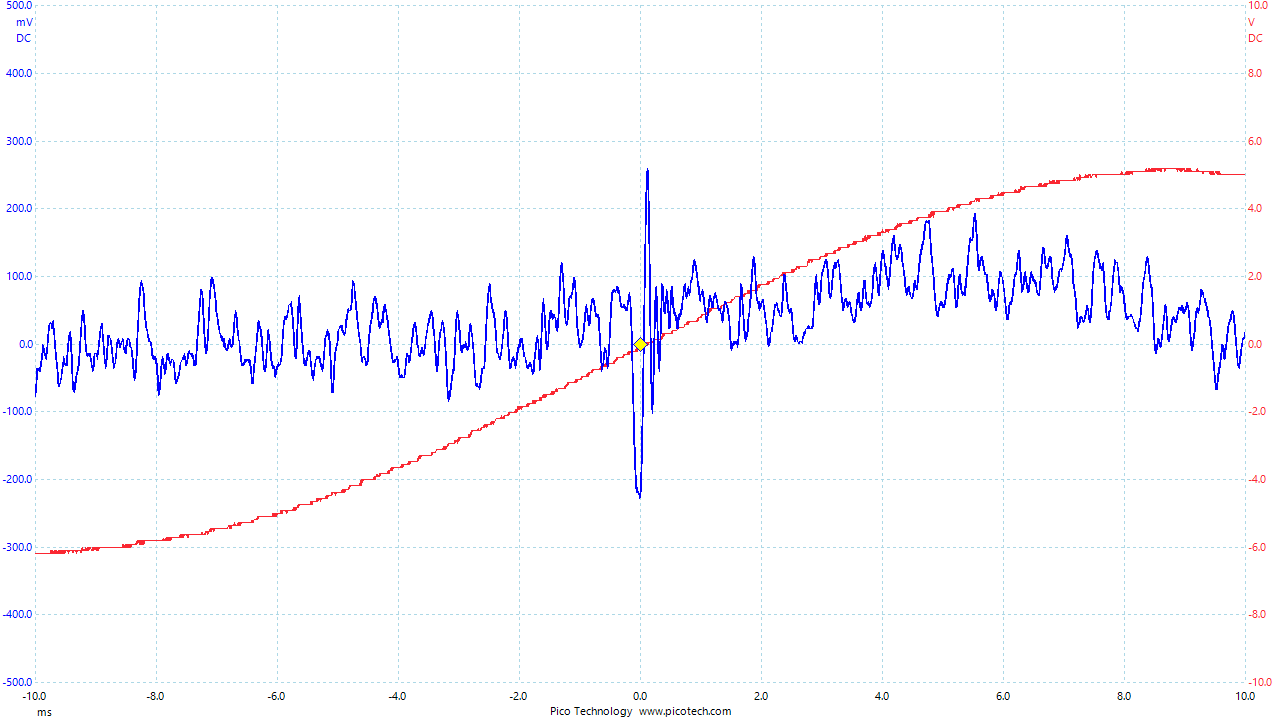
\includegraphics[scale=0.45]{Images/Report/Part A/1A.png}
\caption{An NMR signal of Glycerine with respect with time vs DC voltage.}
\label{Part 1 1A}
\end{figure}

\begin{figure}[H]
\centering
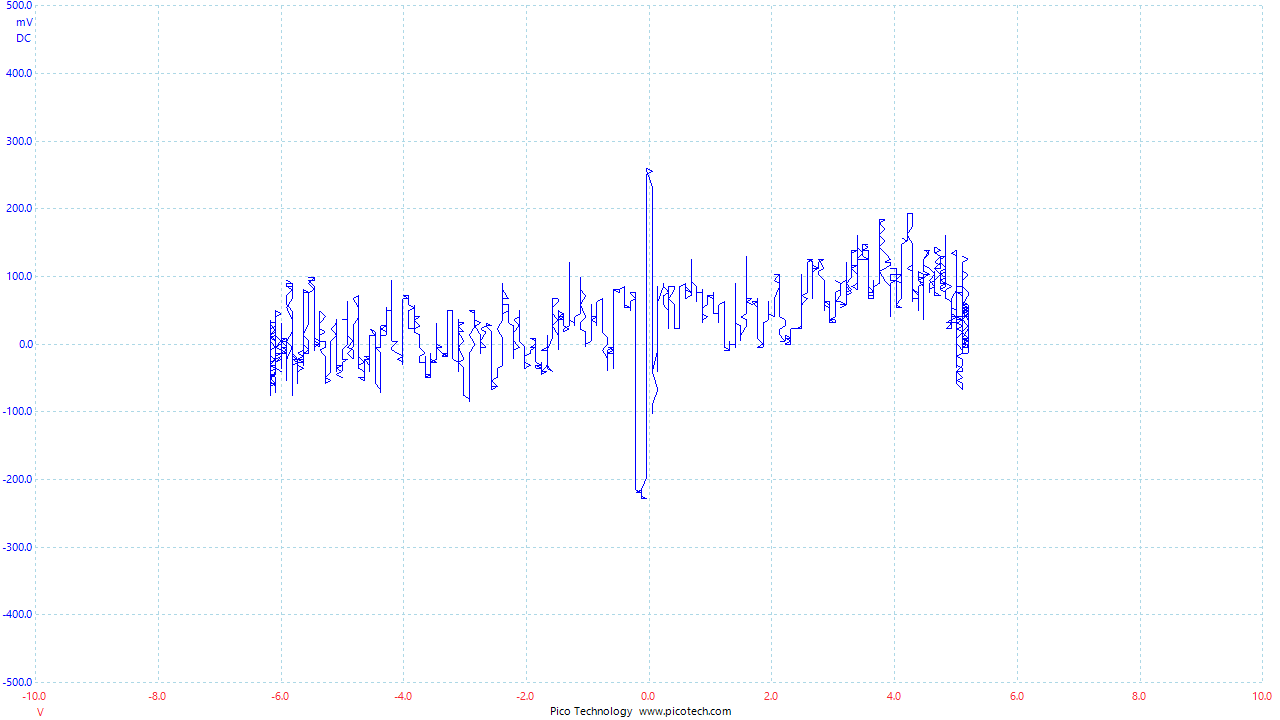
\includegraphics[scale=0.45]{Images/Report/Part A/1B.png}
\caption{An NMR signal of Glycerine with respect with magnetic field strength vs DC voltage.}
\label{Part 1 1B}
\end{figure}

\begin{figure}[H]
\centering
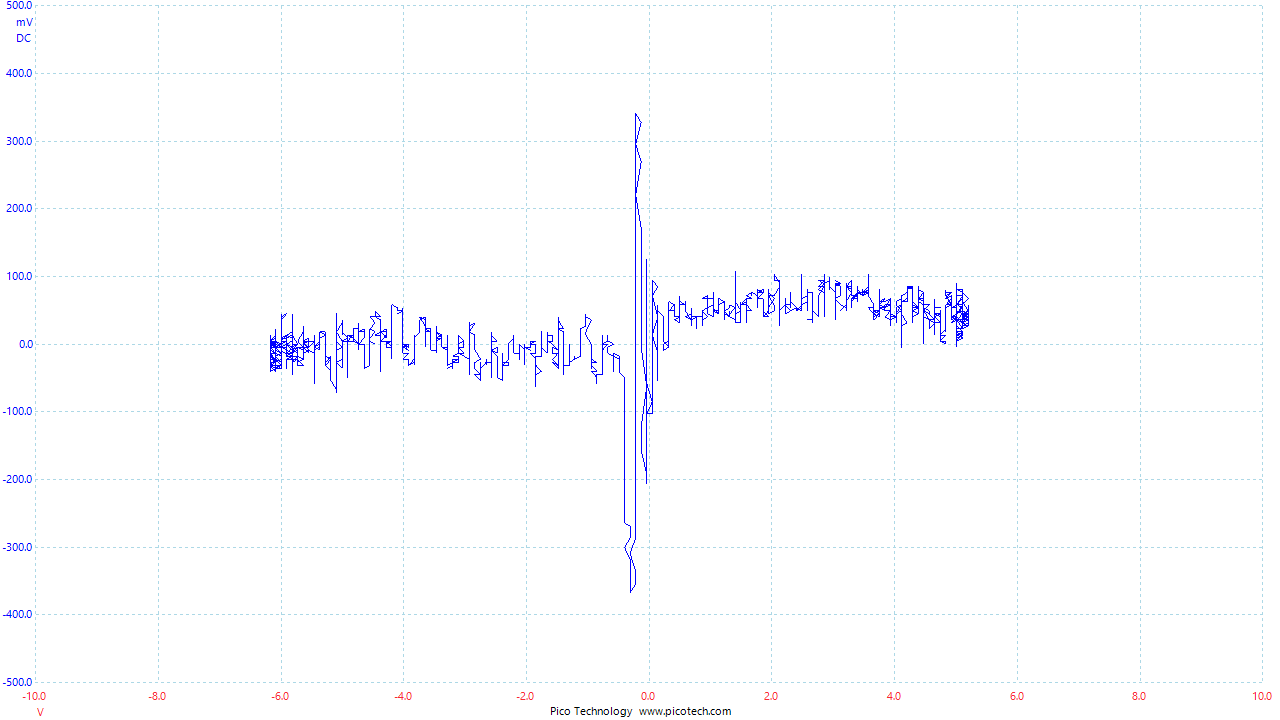
\includegraphics[scale=0.45]{Images/Report/Part A/2B.png}
\caption{An NMR signal of Water with respect with magnetic field strength vs DC voltage.}
\label{Part 1 2B}
\end{figure}

\begin{figure}[H]
\centering
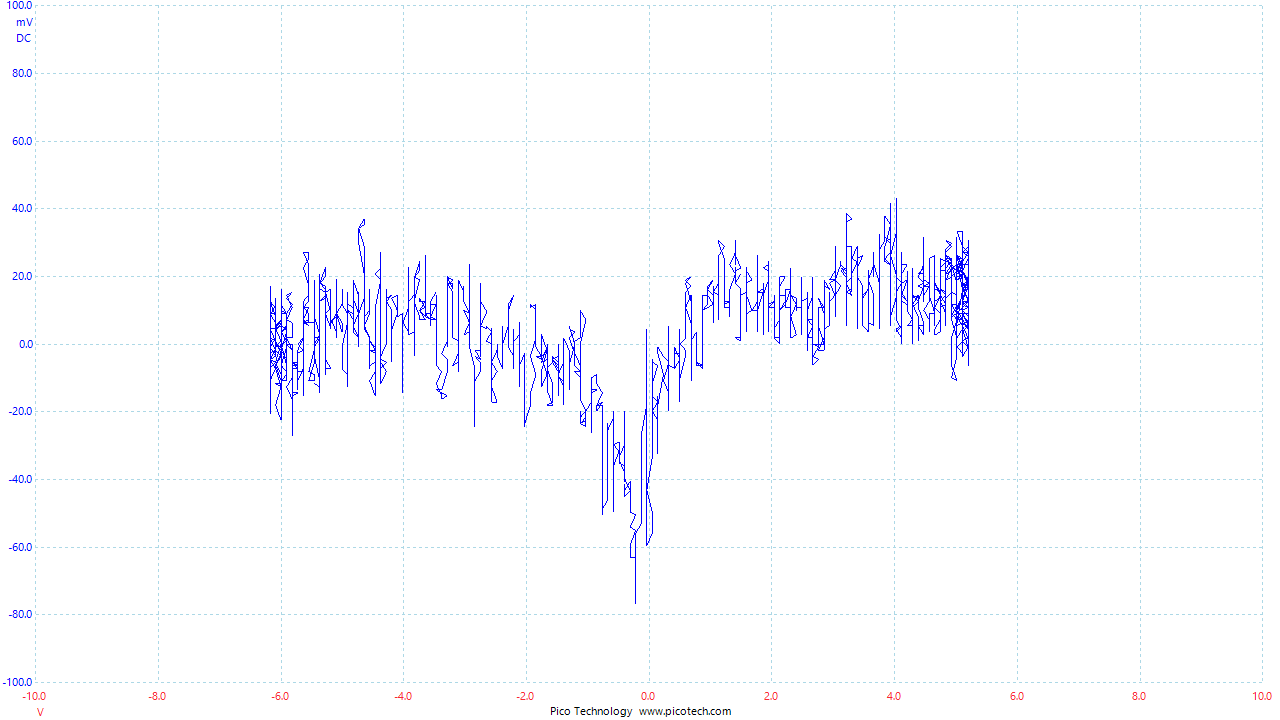
\includegraphics[scale=0.45]{Images/Report/Part A/3B.png}
\caption{An NMR signal of Polystyrene with respect with magnetic field strength vs DC voltage.}
\label{Part 1 3B}
\end{figure}

\begin{figure}[H]
\centering
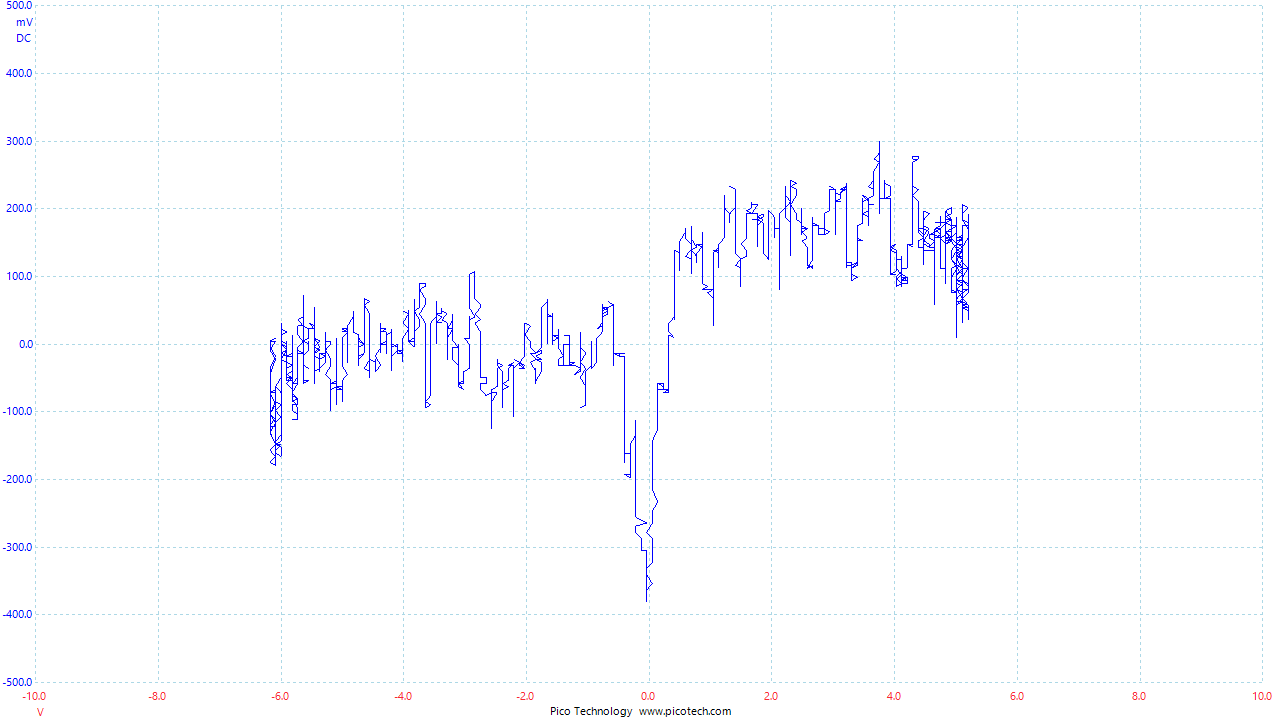
\includegraphics[scale=0.45]{Images/Report/Part A/4B.png}
\caption{An NMR signal of PTFE with respect with magnetic field strength vs DC voltage.}
\label{Part 1 4B}
\end{figure}

\begin{figure}[H]
\centering
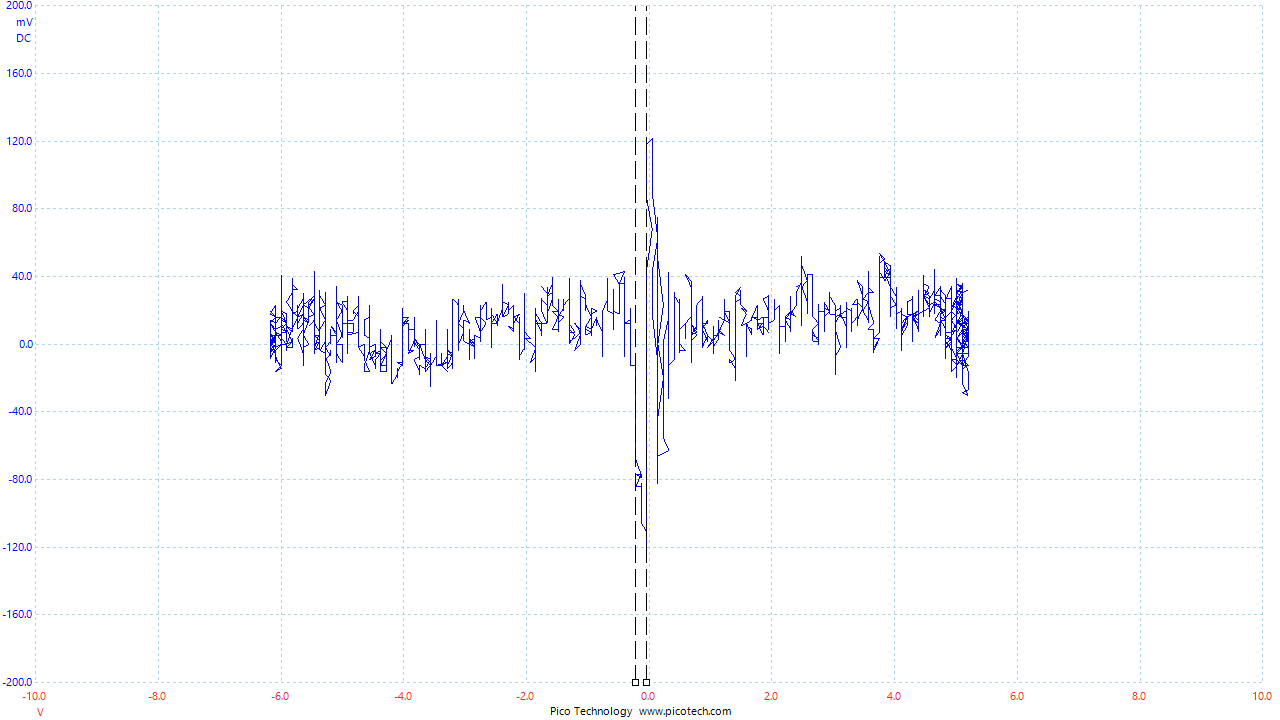
\includegraphics[scale=0.45]{Images/Report/Part A/Linewidth.png}
\caption{An NMR signal of glycerine and using the PicoScope software, the determination of linewidth is found.}
\label{Linewidth}
\end{figure}

%---------------------------------------------------------------------------
\subsection{Chemical NMR Spectroscopy}
\label{Chemical NMR Spectroscopy SubSection}

Moving into the Chemical spectroscopy of Nuclear Magnetic Resonance (NMR), the signal was prefixed to detect glycerine before the hand cream sample replaced the glycerine sample. Little shift in frequency and RF amplitude was introduced when comapring the glycerine data (\cref{Phy NMR Spec} and the hand cream data(\cref{Chem NMR Spec}), to reduce the signal/ noise ratio and comparing \cref{Part 1 5B} to \cref{Part 1 1B} show similarities in the Nuclear Magnetic Resonance (NMR) signals wave structure but lowers and raises in the negative/ positive magnetic field strength, the peaks of the NMR signal are around fours times more in frequency than in the original glycerine sample showing that the glycerine nuclei have been detected at a larger quantity but are more sensitive to the external magnetic field. Indicating that other elements in the hand cream cause the glycerine nuclei to react differently that when the glycerine nuclei are on their own. \\

\begin{table}[H]
\begin{center}
 \footnotesize
 \begin{tabular}{|c||c||c||c||c|}
 \hline
 \multicolumn{5}{|c|}{Nuclear Magnetic Resonance (NMR) of water protons in hand cream in a chemical aspect of this experiment} \\
 \hline
 Material & Frequency (MHz)  & Current (Amps)  & Voltage (V) & Standard Deviation \\
 \hline \hline
 Hand Cream & 17.6504 $\pm$0.0001  & 3.18 $\pm$0.01  & 7.9 $\pm$0.1 & 7.379\\
 \hline
 \end{tabular} \\ 
 \caption{Variable data collected from the NMR signal of the glycerine in hand cream for chemical NMR spectroscopy.}
 \label{Chem NMR Spec}
\end{center}
\end{table}

\begin{figure}[H]
\centering
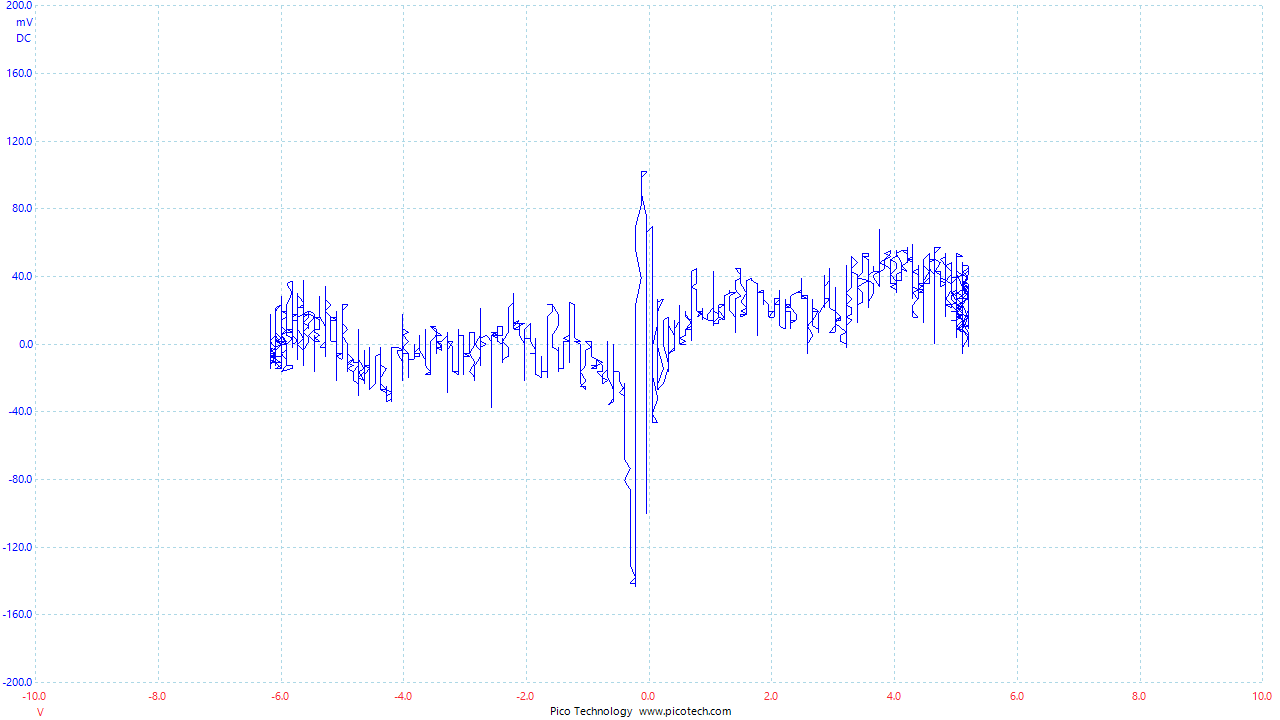
\includegraphics[scale=0.45]{Images/Report/Part A/5B.png}
\caption{An NMR signal of glycerine in Hand Cream with respect with magnetic field strength vs DC voltage.}
\label{Part 1 5B}
\end{figure}

%---------------------------------------------------------------------------
\subsection{Biological NMR Spectroscopy}
\label{Biological NMR Spectroscopy SubSection}

Again but finding the Nuclear Magnetic Resonance (NMR) signal for water first before changing to the fresh grass sample, again small shift in frequency and RF amplitude as shown in \cref{Phy NMR Spec} and \cref{Bio NMR Spec} to the water and grass sample shows that \cref{Part 1 6B} is displaying the water molecules in the fresh grass sample. Comparing the grass sample (\cref{Part 1 6B}) the the water sample (\cref{Part 1 2B}) shows almost the exact amount of water in the grass sample as the standalone water sample if not slightly lower, when the grass was pick it was raining so the excess or equal water molecules can be explained. Though the peaks aren't as intense as they are in the grass sample as in the water sample, the relative shape of the Nuclear Magnetic Resonance (NMR) signal is the same allowing the determination of the conclusion that isolating the specific water molecules in freshly cut grass is appropriate. \\ 

\begin{table}[H]
\begin{center}
 \footnotesize
 \begin{tabular}{|c||c||c||c||c|}
 \hline
 \multicolumn{5}{|c|}{Nuclear Magnetic Resonance (NMR) of water protons in grass for biological NMR spectroscopy} \\
 \hline
 Material & Frequency (MHz)  & Current (Amps)  & Voltage (V) & Standard Deviation \\
 \hline \hline
 Grass & 17.6101 $\pm$0.0001  & 3.15 $\pm$0.01  & 7.9 $\pm$0.1 & 7.370\\
 \hline
 \end{tabular} \\ 
 \caption{Variable data collected from the NMR signal of the water in grass for biological NMR spectroscopy.}
 \label{Bio NMR Spec}
\end{center}
\end{table}

\begin{figure}[H]
\centering
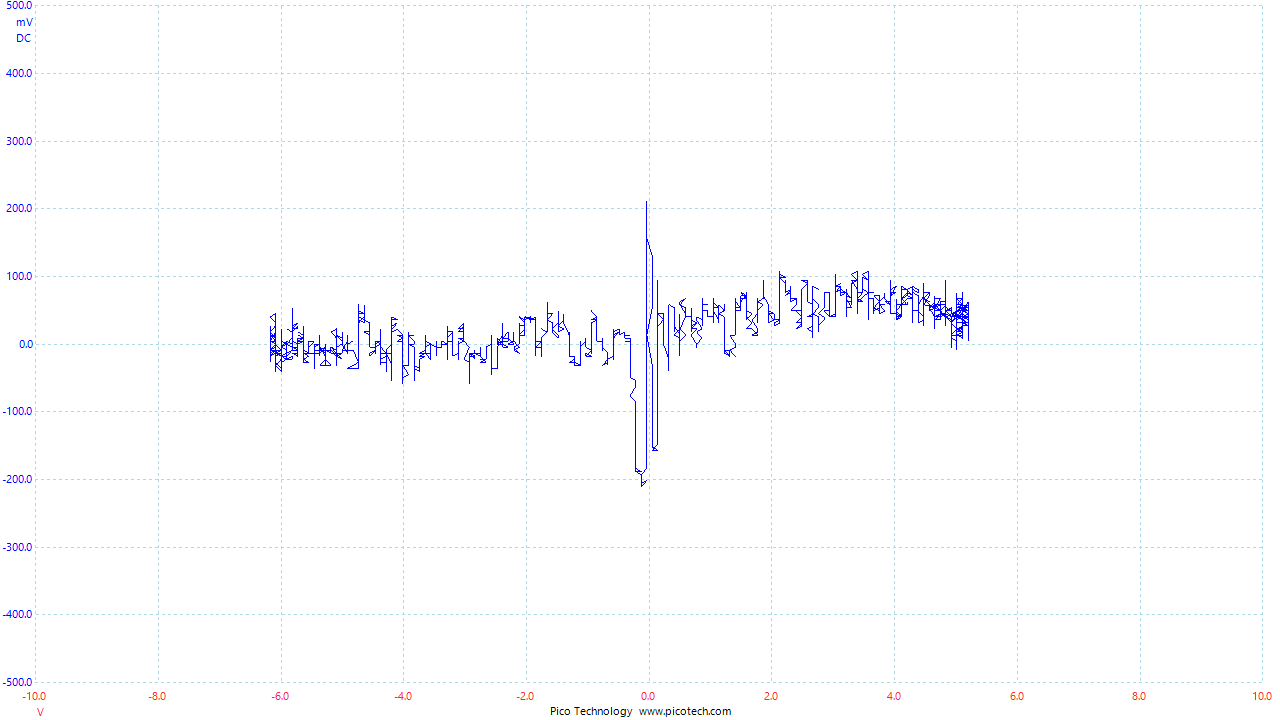
\includegraphics[scale=0.45]{Images/Report/Part A/6B.png}
\caption{An NMR signal of water in fresh grass with respect with magnetic field strength vs DC voltage.}
\label{Part 1 6B}
\end{figure}

%---------------------------------------------------------------------------
\subsection{Determination of the g-factor}
\label{Determination of the g-factor SubSection}

By repeating the experiment and altering the current in a positive and negative of the 3.2 Amps set up and thus changing the RF amplitude and frequency, multiple Nuclear Magnetic Resonance (NMR) signals can be found and observed, the data collect for the samples of glycerine and PTFE in \cref{Gly NMR Spec} and \cref{PTFE NMR Spec} shows the collected data of Frequency, Current, Voltage and Magnetic field strength. The NMR signal was found and the smaple taken out and a Combi B-sensor S was implanted in the centre of the magnetic field in which the NMR signal was found and the fields strength was measured. \\

\begin{table}[H]
\begin{center}
 \footnotesize
 \begin{tabular}{|c||c||c||c||c|}
 \hline
 \multicolumn{5}{|c|}{Data set for the NMR signal of Glycerine at variable frequencies} \\
 \hline
 Frequency (MHz)  & Current (Amps)  & Voltage (V) & Standard Deviation & Magnetic Field (mT)\\
 \hline \hline
 16.2015 $\pm$0.0001  & 2.82 $\pm$0.01  & 7.6 $\pm$0.1 & 7.075 &  -396 $\pm$2 \\
 \hline
 16.5451 $\pm$0.0001  & 2.90 $\pm$0.01  & 7.2 $\pm$0.1 & 7.132 &  -405 $\pm$2 \\
 \hline
 17.0254 $\pm$0.0001  & 3.00 $\pm$0.01  & 7.4 $\pm$0.1 & 7.429 &  -416 $\pm$2 \\
 \hline
 17.3603 $\pm$0.0001  & 3.10 $\pm$0.01  & 7.7 $\pm$0.1 & 7.573 &  -425 $\pm$2 \\
 \hline
 17.7071 $\pm$0.0001  & 3.20 $\pm$0.01  & 7.6 $\pm$0.1 & 7.711 &  -433 $\pm$2 \\
 \hline
 18.0530 $\pm$0.0001  & 3.30 $\pm$0.01  & 8.0 $\pm$0.1 & 7.075 &  -442 $\pm$2 \\
 \hline
 18.3860 $\pm$0.0001  & 3.41 $\pm$0.01  & 8.4 $\pm$0.1 & 8.006 &  -448 $\pm$2 \\
 \hline
 18.6263 $\pm$0.0001  & 3.49 $\pm$0.01  & 8.6 $\pm$0.1 & 8.108 &  -457 $\pm$2 \\
 \hline
 19.1858 $\pm$0.0001  & 3.63 $\pm$0.01  & 8.5 $\pm$0.1 & 8.334 &  -469 $\pm$2 \\
 \hline
 \end{tabular} \\ 
 \caption{}
 \label{Gly NMR Spec}
\end{center}
\end{table}

\begin{table}[H]
\begin{center}
 \footnotesize
 \begin{tabular}{|c||c||c||c||c|}
 \hline
 \multicolumn{5}{|c|}{Data set for the NMR signal of PTFE at variable frequencies} \\
 \hline
 Frequency (MHz)  & Current (Amps)  & Voltage (V) & Standard Deviation & Magnetic Field (mT)\\
 \hline \hline
 16.8500 $\pm$0.0001  & 2.96 $\pm$0.01  & 7.5 $\pm$0.1 & 6.908 &  -412 $\pm$2 \\
 \hline
 16.2496 $\pm$0.0001  & 3.09 $\pm$0.01  & 7.6 $\pm$0.1 & 7.069 &  -423 $\pm$2 \\
 \hline
 16.6202 $\pm$0.0001  & 3.21 $\pm$0.01  & 8.2 $\pm$0.1 & 7.242 &  -432 $\pm$2 \\
 \hline
 17.0770 $\pm$0.0001  & 3.34 $\pm$0.01  & 8.5 $\pm$0.1 & 7.438 &  -441 $\pm$2 \\
 \hline
 17.4458 $\pm$0.0001  & 3.45 $\pm$0.01  & 8.7 $\pm$0.1 & 7.593 &  -453 $\pm$2 \\
 \hline
 17.7255 $\pm$0.0001  & 3.56 $\pm$0.01  & 9.0 $\pm$0.1 & 7.715 &  -462 $\pm$2 \\
 \hline
 18.1699 $\pm$0.0001  & 3.67 $\pm$0.01  & 9.2 $\pm$0.1 & 7.903 &  -471 $\pm$2 \\
 \hline
 18.5156 $\pm$0.0001  & 3.77 $\pm$0.01  & 9.4 $\pm$0.1 & 8.049 &  -482 $\pm$2 \\
 \hline
 18.8067 $\pm$0.0001  & 3.87 $\pm$0.01  & 9.6 $\pm$0.1 & 8.173 &  -487 $\pm$2 \\
 \hline
 19.1192 $\pm$0.0001  & 3.99 $\pm$0.01  & 10.1 $\pm$0.1 & 8.322 &  -496 $\pm$2 \\
 \hline
 \end{tabular} \\ 
 \caption{}
 \label{PTFE NMR Spec}
\end{center}
\end{table}

Determining the g-factor means plotting the frequency in Hertz against the magnetic field strength in Telsa. Shown for glycerine in \cref{Part B2} and for PTFE in \cref{Part B1}, a line of best fit was applied to the data linearly to achieve the g-factor for glycerine which was $-2x10^{-8}$ and for PTFE was $-3x10^{-8}$. The literature values calculated using;

\begin{equation}
g= \dfrac{h*v}{U_n * B_o}
\label{Log Tramsittance 1}
\end{equation}

Where h is Plancks constant of $6.626x10^{-34}$ J s and v the frequency, $U_n$ is the nuclear magneton of a value $5.051x10^{-27}$ J/T and $B_o$ the magnetic field strength. The literature values were calculated at for glycerine is $g_g=-5.37$ and for PTFE $g_g=-5.05x10^{-3}$. \\

When comparing the experimental values to the calculated literature value, the early statement arises from the line width where this experiment is a much smaller and low strength experiment, thus an assumption could be made that the discrepancy between the two values could be stated as a flaw due to apparatus quality restrictions. The linearity of both \cref{Part B2} and \cref{Part B1} shows the experimental data forming a relationship between frequency and the magnetic field strength but thus the literature values two of which are constants (the Planck's constant and the nuclear magneton) wither shows a human error or an experimental error. \\

\begin{figure}[H]
\centering
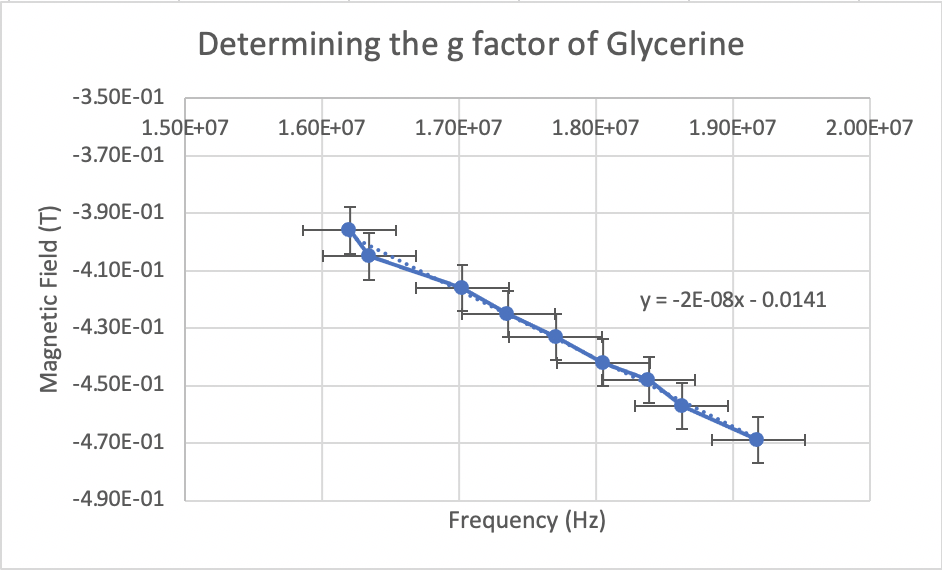
\includegraphics[scale=0.8]{Images/Report/Part B1/Screenshot 2020-12-02 at 20.43.19.png}
\caption{Graphical plot of collected glycerine data from \cref{Gly NMR Spec} plotting frequency against the strength of the magnetic field.}
\label{Part B2}
\end{figure}

\begin{figure}[H]
\centering
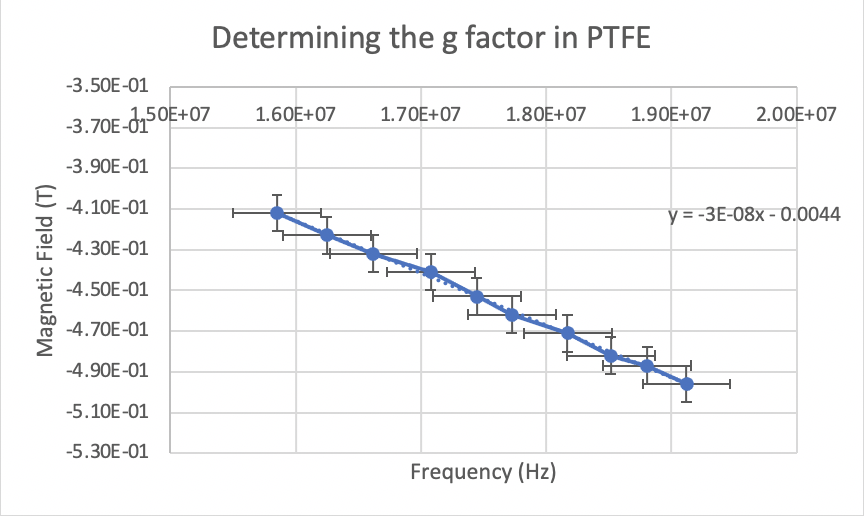
\includegraphics[scale=0.8]{Images/Report/Part B1/Screenshot 2020-12-02 at 20.45.58.png}
\caption{Graphical plot of collected PTFE data from \cref{PTFE NMR Spec} plotting frequency against the strength of the magnetic field.}
\label{Part B1}
\end{figure}

%---------------------------------------------------------------------------
%	DISCUSSION
%---------------------------------------------------------------------------
\section{Discussion}
\label{Disscussion Section}

This experiment i believe to be a success, the calculated line width was accurate enough to describe the apparatus restrictions when comparing to the $T_2$ relaxation line width, this is shown also in the PicoScope where only one visible Nuclear Magnetic Resonance (NMR) signal was discovered at any one time where as if the equipment was improved and a larger/ stronger magnetic field was applied the waveform would show multiple NMR signals, thus showing the individual protons of the nuclei. Moving into the chemical and biological spectroscopy, the experiment showed that pre-setting the sample i.e. glycerine and water almost immediately detected in the hand cream and the fresh grass thus showing the that in the medical world, magnetic resonance imaging (MRI) can pick out certain molecules if pre selected. \\

Moving on the the g-factor, i believe a mixture of human error in the calculating the literature value was to blame but its important to not forget that the experimental apparatus is limited as defined in the the line width calculation. This leads me on to my next point, i believe that sourcing multiple data i.e. the frequency, current and voltage again would correct this flaw as the more data to work with would produce more accurate results. 

%---------------------------------------------------------------------------
%	CONCLUSION
%---------------------------------------------------------------------------
\section{Conclusion}
\label{Conclusion Section}

In conclusion, the Nuclear Magnetic Resonance (NMR) signals were all found and the line width calculation of 4.422 kHZ for the experimental data vs the calculated relaxation of glycerine at 637.42 Hz is explained due to apparatus restrictions. Proved the use of Nuclear Magnetic Resonance (NMR) in chemistry and biology by pre-fixing the NMR signal on a isolated sample which allows the observation of glycerine and water in hand cream and fresh grass. This further explored the physical and biological use behind magnetic resonance imaging (MRI). The g-factor values did not match at all, though a plausible explanation could be that of apparatus restrictions much like the line width calculation but human error attributed to this. Further analysis should be required but the aims where met and achieved.

%---------------------------------------------------------------------------
%	APPENDIX
%---------------------------------------------------------------------------
\newpage
\section{Appendix}
\label{Appendix Section}

\begin{figure}[H]
\centering
\includegraphics[scale=0.25]{Images/Labbook/IMG_0492.PNG}
\end{figure}
\newpage
\begin{figure}[H]
\centering
\includegraphics[scale=0.25]{Images/Labbook/IMG_0493.PNG}
\end{figure}
\newpage
\begin{figure}[H]
\centering
\includegraphics[scale=0.25]{Images/Labbook/IMG_0494.PNG}
\end{figure}
\newpage
\begin{figure}[H]
\centering
\includegraphics[scale=0.25]{Images/Labbook/IMG_0495.PNG}
\end{figure}
\newpage
\begin{figure}[H]
\centering
\includegraphics[scale=0.25]{Images/Labbook/IMG_0496.PNG}
\end{figure}
%---------------------------------------------------------------------------
%	REFERENCES
%---------------------------------------------------------------------------
\bibliographystyle{plain}
\bibliography{mybib.bib}
\end{document}